\section{Image Analysis}

In order to assess the potential for coalescing duplicated data between
virtual disk images we compared a cross-section of images from various 
versions of various Linux distributions as well images resulting from
separate installs of Windows XP.
We establish overlap candidates by crawling the file systems, producing a SHA-1
cryptographic hash for each file and associating it with the size of the 
file and the number of hard-links to the file in a manner similar to
Mirage's manifests~\cite{mirage}.
The Linux file systems in question are Ext2 formatted root volumes
(without /boot which contains the kernels and ram disks) present after the 
default installation of the various distributions.

We then determine the amount of self-similarity within a file system by looking
for duplicate hashes and discounting hard linked copies as false duplicates.
Our analysis showed that typical root disk images have around 5\% 
duplicate file data within a single image after initial installation, 
and that the amount of duplicate file data seems to be increasing 
(Fedora 7 had 4.1\% or 70MB, Fedora 9 has 5.3\% or 116MB).
We then concatenate file lists from two different images and look for
duplicate file hashes to establish the amount of data duplicated between
the two images.  The total size of the duplicate files is compared to the
total size of all files from the two images to calculate the \% of duplicates.

\begin{figure}[htbp]
\begin{centering}
\begin{tabular}{|l|r|r|r|r|}	\hline 
\emph{Image}	& Base	& Office	& SDK	& Web \\ \hline
Base	& 96\%	& 88\%	& 85\%	& 95\% \\
Office	& 	& 96\%	& 79\%	& 87\% \\
SDK	& 	& 	& 96\%	& 85\% \\
Web	& 	& 	& 	& 96\% \\	\hline
\end{tabular}
\small\itshape
\caption{\small\itshape Different Fedora 9 Flavors}
\label{fig:flavors}
\end{centering}
\end{figure}

Figure~\ref{fig:flavors} shows the amount of similarity between
separate installs of several different configurations of the Fedora 9
x86--64 distribution.  The image personality is determined by options
selected during the installation process.
The \emph{Base} configuration is the 
standard installation, with no personality configuration selected.
The \emph{Office} configuration contains productivity applications such
as OpenOffice, the \emph{SDK} configuration contains development tools
and resources, and the \emph{Web} configuration contains the necessary
applications for web serving.
Separate installations of the same configuration had 96\% similarity 
according to our methodology.  The differences are likely log files and
other metadata which would be particular to a specific system instance.
Not surprisingly, the similarity amongst the different configurations is 
relatively high due to the common base installation which accounts for 
around 80\% or more of the data.

\begin{figure}[htbp]
\begin{centering}
\resizebox{\columnwidth}{!}
{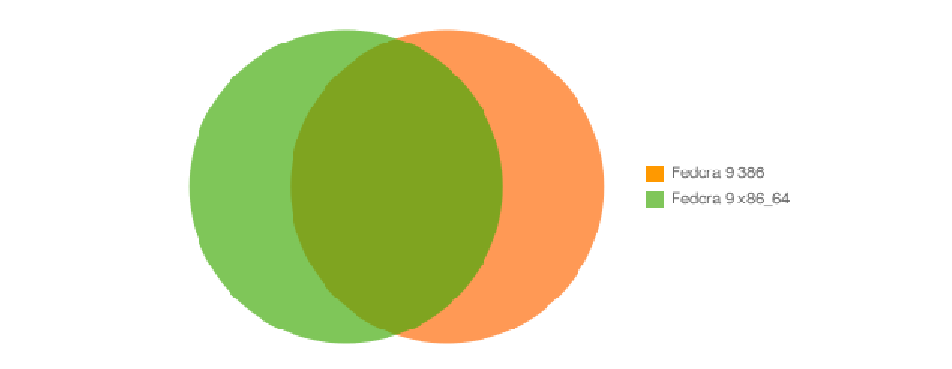
\includegraphics{fedorax86}}
\small\itshape
\caption{\small\itshape Different Architectures}
\label{fig:arch}
\end{centering}
\end{figure}

We then compared slightly less similar images by
comparing the installation of a 32-bit Fedora 9 system with
a 64-bit Fedora 9 system.  As can be seen in Figure~\ref{fig:arch}
we observed roughly 60\% overlap between the two images consisting 
primarily of the non-binary portions of the installation (configuration
files, fonts, icons, documentation, etc.).

\begin{figure}[htbp]
\begin{centering}
\begin{tabular}{|l|r|r|r|r|r|}	\hline 
\emph{Image}	& Fed 8	& Fed 9	& Ubuntu	& OpenSuSe-11	\\ \hline
Fedora 7 	& 34\%	& 22\%	&  8\%	& 15\% \\
Fedora 8 	& 	& 31\%	& 10\%	& 16\% \\
Fedora 9	& 	& 	& 11\%	& 21\% \\
Ubuntu 8.04	& 	& 	& 	& 8\% \\	\hline
\end{tabular}
\small\itshape
\caption{\small\itshape Different Distributions}
\label{fig:distro}
\end{centering}
\end{figure}

Next, we compared several different distributions, looking at the overlap
between different versions of Fedora as well as 32-bit versions of
Ubuntu and OpenSuSe 11.
The resulting overlap can be seen in Figure~\ref{fig:distro}. 
As one might expect, adjacent versions of the distribution had relatively
high degrees of overlap ranging from 22\% to 34\% despite about a year of
time between their respective releases.
It should be pointed out that the effect is cumulative, if looking across 
all three distributions which total about 6 GB of root file system data, 
2GB of that data is overlapped data resulting in approximately 1.2GB of
wasted space.
The overlap between the Fedora installations and the other distribution
vendors is less striking.  There was a high degree of overlap between 
Fedora and OpenSuSe but a much lower degree of overlap with Ubuntu.
The results are a little offset because the Ubuntu image is almost an
order of magnitude smaller than the Fedora and SuSe base installations.

\begin{figure}[htbp]
\begin{centering}
\resizebox{\columnwidth}{!}
{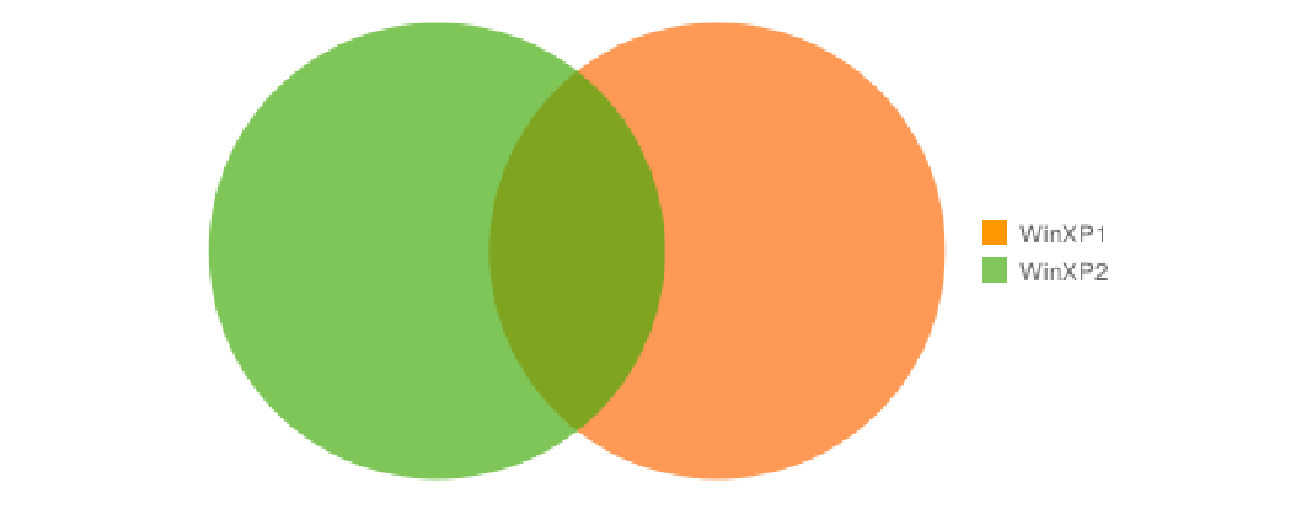
\includegraphics{winxp}}
\small\itshape
\caption{\small\itshape Individual WindowsXP Installs}
\label{fig:windows}
\end{centering}
\end{figure}

Switching from Linux to Windows, we compared two separate installations
of WindowsXP on a FAT32 file system. 
We selected a FAT32 installation over NTFS to reduce the complexity of
analyzing block-based results.
We were somewhat dismayed to discover only a 27\% overlap as can be seen
in Figure~\ref{fig:windows}.
A closer look reveals that the two largest files in the instance file systems
are the hibernation file (\emph{hiberfil.sys}) clocking in at just under
a gigabyte in size and the swap file (\emph{pagefile.sys}) hovering around
1.5 gigabytes in size.  This 2.5 gigabytes actually comprises more then 60\%
of the overall size of the file system.  Discounting these two files we find
roughly 90\% overlap between the two distributions.

\begin{figure}[htbp]
\begin{centering}
\resizebox{\columnwidth}{!}
{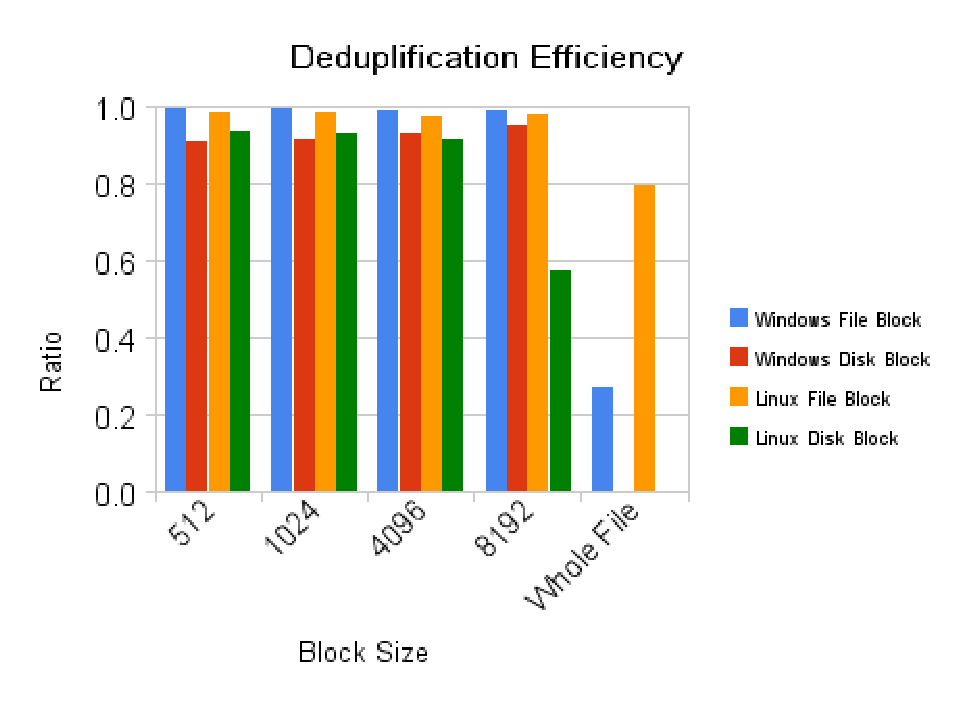
\includegraphics{deduplification_efficiency}}
\small\itshape
\caption{\small\itshape Effect of Block Size on Efficiency}
\label{fig:block}
\end{centering}
\end{figure}

Digging deeper, we observed that both of these files were primarily 
zero--filled.
We reworked our analysis tools to perform block-level hashing of files
within the file system at 512-byte, 1k, 4k, and 8k granularities.
By comparing file content hashes at this level of granularity we were
able to more effectively detect duplication within files as well as 
handle sparse files more efficiently.  As can be seen in the 
\emph{Windows File Block} results in Figure~\ref{fig:block} we achieved near
perfect (99\%) de-duplification of the two Windows install images using
any of the block size options.  Results were fractional better with 512
byte blocks, but the overhead associated with tracking such small blocks
in a CAS would far outweigh the benefits.

We also used the same tool to scan the raw disk image at the
various block granularities.  Its effectiveness at de-duplicating blocks
are shown in the \emph{Windows Disk Block} result in Figure~\ref{fig:block}.
The results show a slightly higher efficiency for 8k blocks, but this is
primarily due to error associated with partial blocks and our discounting
zero-filled-blocks.  The disk based scan was able to identify approximately
93\% of the duplicate data.

We then applied these same two techniques to analyzing two different
installations of the same Linux distribution as can be seen in the
\emph{Linux File Block} and \emph{Linux Disk Block} results.  We found
similar results to the Windows analysis with the exception that 8k
block granularity did very poorly with Linux most likely due to differences
between Ext2 and FAT32 layout schemes since both file systems reported using
4k block sizes.

